\documentclass[11pt]{article}

\usepackage[margin=1in]{geometry}
\usepackage[T1]{fontenc}
\usepackage[utf8]{inputenc}
\usepackage{lmodern}
\usepackage{booktabs}
\usepackage{tabularx}
\usepackage{array}
\usepackage{enumitem}
\usepackage{hyperref}
\usepackage[dvipsnames]{xcolor}
\usepackage{tikz}
\usepackage{graphicx}
\usepackage{titlesec}
\usepackage{fancyhdr}

\usetikzlibrary{arrows.meta, positioning, shapes.geometric, shapes.multipart}

\hypersetup{
  colorlinks=true,
  linkcolor=MidnightBlue,
  urlcolor=MidnightBlue,
  pdftitle={Home Credit Default Risk Case Justification},
  pdfauthor={OpenAI Codex}
}

\setlength{\parindent}{0pt}
\setlength{\parskip}{0.65em}
\setlength{\headheight}{14pt}
\emergencystretch=1em
\setlist[itemize]{topsep=0.35em, itemsep=0.2em, leftmargin=1.2em}
\setlist[enumerate]{topsep=0.35em, itemsep=0.2em, leftmargin=1.4em}

\definecolor{CaseInk}{HTML}{1C1713}
\definecolor{CaseAccent}{HTML}{8C5638}
\definecolor{CaseMoss}{HTML}{5E664C}
\definecolor{CaseSoft}{HTML}{F4EEE6}
\definecolor{CaseLine}{HTML}{D8C8B7}

\titleformat{\section}{\Large\bfseries\color{CaseInk}}{\thesection.}{0.6em}{}
\titleformat{\subsection}{\large\bfseries\color{CaseInk}}{\thesubsection.}{0.6em}{}

\pagestyle{fancy}
\fancyhf{}
\fancyhead[L]{Home Credit Case Justification}
\fancyhead[R]{Explainable Credit Risk}
\fancyfoot[C]{\thepage}

\newcommand{\metric}[2]{\textbf{#1}: #2}
\newcolumntype{Y}{>{\raggedright\arraybackslash}X}
\newcolumntype{P}[1]{>{\raggedright\arraybackslash}p{#1}}

\begin{document}

{\Huge\bfseries Designing an Explainable Credit Risk Stack\par}
{\Large Home Credit Default Risk Case Justification\par}
\vspace{0.5em}
{\large A LaTeX case note for interview use, portfolio discussion, and model-defense discussion.\par}
\vspace{0.75em}

\begin{tabularx}{\textwidth}{@{}YY@{}}
\metric{Dataset}{Kaggle Home Credit Default Risk competition, focused on predicting repayment difficulty for consumer borrowers.} &
\metric{Competition Link}{\url{https://www.kaggle.com/competitions/home-credit-default-risk/}} \\
\metric{Primary modeling path}{Explainable scorecard built on WoE / IV logic, reason codes, and PSI-style monitoring.} &
\metric{Secondary benchmark}{Leaderboard-style ensemble used as a performance reference, not the main operating surface.}
\end{tabularx}

\vspace{1em}

\section{Executive Summary}

This case is easiest to defend when it is framed as a credit-risk system rather than as a Kaggle model. The project does four things:

\begin{itemize}
  \item It organizes the problem around the core lending question: can this borrower repay, and will this borrower repay?
  \item It turns a multi-table credit dataset into a curated feature layer that supports both portfolio analysis and scoring.
  \item It prioritizes an explainable scorecard with reason codes and drift diagnostics over a pure black-box presentation.
  \item It closes the loop from book-level monitoring to borrower-level traceability, which is the right way to discuss production credit AI.
\end{itemize}

The strongest business result is not only that the scorecard performs well, but that it remains operationally explainable:

\begin{center}
\begin{tabular}{@{}lccccccc@{}}
\toprule
Metric & ROC AUC & KS & PR AUC & Brier & Features & Train Mon. & Test Mon. \\
\midrule
Scorecard & 0.8556 & 0.5801 & 0.4654 & 0.0580 & 23 & 1{,}000 & 20{,}000 \\
\bottomrule
\end{tabular}
\end{center}

\section{Portfolio Snapshot and Data Reality}

The competition is a binary default-risk problem over a large, heterogeneous consumer-lending portfolio. The first thing to establish in an interview is that this is not a clean single-table classification task. It is a multi-table underwriting environment with application data, bureau data, prior internal applications, POS history, card behavior, and installment behavior. That matters because the project's main lift comes from translating those raw tables into a coherent credit view.

\begin{center}
{\small
\begin{tabularx}{\textwidth}{@{}P{0.24\textwidth}P{0.12\textwidth}Y@{}}
\toprule
Portfolio fact & Value & Why it matters \\
\midrule
Training rows & 307{,}511 & Large enough to support robust feature screening and scorecard validation \\
Default rate & 8.0729\% & Meaningfully imbalanced, so PR AUC and KS matter alongside ROC AUC \\
Baseline analysis ROC AUC & 0.6292 & Raw portfolio signals are useful, but insufficient without domain feature engineering \\
Baseline analysis PR AUC & 0.1529 & Establishes the gap between naive modeling and a deployable scorecard \\
\bottomrule
\end{tabularx}
}
\end{center}

This framing is important for two reasons:

\begin{itemize}
  \item \textbf{Credit data is layered.} Capacity lives mainly in the application. Willingness lives mainly in historical behavior.
  \item \textbf{Credit data is messy.} Special values, missing bureau fields, uneven table coverage, and changing applicant mix are part of the real modeling problem.
\end{itemize}

\section{A Clean Way to Explain the Project}

To keep the project mutually exclusive in scope and collectively exhaustive in coverage, it helps to explain it through four non-overlapping lenses:

\begin{enumerate}
  \item \textbf{Portfolio and data conditions} --- what kind of risk pool is being modeled, and what data limitations are present.
  \item \textbf{Risk logic} --- the causal credit ideas that make the features economically meaningful.
  \item \textbf{Model stack} --- how the feature layer becomes an explainable scorecard and a benchmark ensemble.
  \item \textbf{Governance and traceability} --- how outputs are monitored, explained, and rendered for a single borrower.
\end{enumerate}

\subsection{Pyramid Structure}

\begin{center}
\resizebox{\textwidth}{!}{%
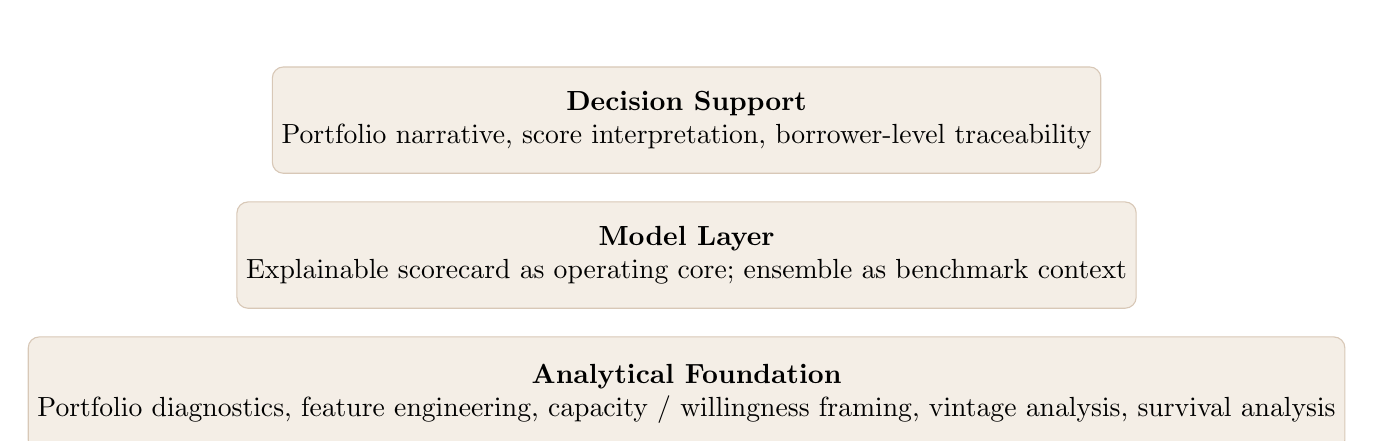
\begin{tikzpicture}[node distance=0.35cm]
  \node[draw=CaseLine, fill=CaseSoft, rounded corners=4pt, minimum width=0.50\textwidth, minimum height=1.35cm, align=center] (top) {
    \textbf{Decision Support}\\
    Portfolio narrative, score interpretation, borrower-level traceability
  };
  \node[draw=CaseLine, fill=CaseSoft, rounded corners=4pt, minimum width=0.72\textwidth, minimum height=1.35cm, align=center, below=of top] (mid) {
    \textbf{Model Layer}\\
    Explainable scorecard as operating core; ensemble as benchmark context
  };
  \node[draw=CaseLine, fill=CaseSoft, rounded corners=4pt, minimum width=0.92\textwidth, minimum height=1.45cm, align=center, below=of mid] (base) {
    \textbf{Analytical Foundation}\\
    Portfolio diagnostics, feature engineering, capacity / willingness framing, vintage analysis, survival analysis
  };
\end{tikzpicture}
}
\end{center}

The pyramid matters because it forces the discussion to start from domain logic and analytical structure before talking about model complexity.

\subsection{System Design Flow}

\begin{center}
\resizebox{\textwidth}{!}{%
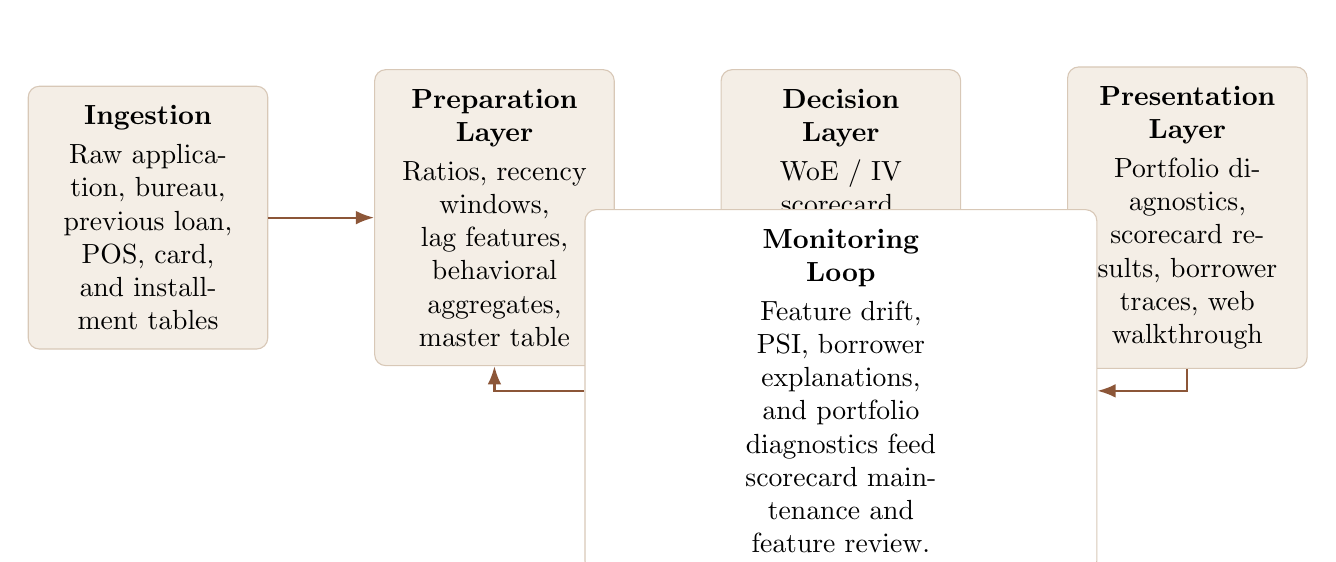
\begin{tikzpicture}[
  box/.style={draw=CaseLine, rounded corners=4pt, fill=CaseSoft, minimum width=2.85cm, minimum height=1.45cm, align=center, inner sep=7pt, text width=2.55cm},
  head/.style={font=\bfseries\small, text=CaseAccent},
  arrow/.style={-Latex, thick, draw=CaseAccent}
]
  \node[box] (ingest1) at (0, 0) {\textbf{Ingestion}\\[2pt]Raw application, bureau, previous loan, POS, card, and installment tables};
  \node[box] (prep1) at (4.4, 0) {\textbf{Preparation Layer}\\[2pt]Ratios, recency windows, lag features, behavioral aggregates, master table};
  \node[box] (decision1) at (8.8, 0) {\textbf{Decision Layer}\\[2pt]WoE / IV scorecard, reason codes, PSI monitoring, benchmark ensemble};
  \node[box] (present1) at (13.2, 0) {\textbf{Presentation Layer}\\[2pt]Portfolio diagnostics, scorecard results, borrower traces, web walkthrough};

  \draw[arrow] (ingest1) -- (prep1);
  \draw[arrow] (prep1) -- (decision1);
  \draw[arrow] (decision1) -- (present1);

  \node[box, minimum width=6.5cm, minimum height=1.15cm, fill=white] (monitor) at (8.8, -2.2) {\textbf{Monitoring Loop}\\[2pt]Feature drift, PSI, borrower explanations, and portfolio diagnostics feed scorecard maintenance and feature review.};
  \draw[arrow] (present1.south) |- (monitor.east);
  \draw[arrow] (monitor.west) -| (prep1.south);
\end{tikzpicture}
}
\end{center}

This is closer to how the project should be discussed in a system-design interview: raw inputs, preparation jobs, decision engines, presentation surfaces, and a monitoring loop.

\section{Why the Credit Framing Is Defensible}

\subsection{The Two-Pillar Starting Point}

Separating \textbf{capacity} from \textbf{willingness} is the right first principle in responsible credit AI.

\begin{itemize}
  \item \textbf{Capacity}: can the borrower afford the obligation? This comes from the application itself: income, loan size, annuity, household burden, and term structure.
  \item \textbf{Willingness}: will the borrower pay even if they can afford it? This comes from repayment history, bureau behavior, prior refusals, and late-payment patterns.
\end{itemize}

These pillars should not be substituted for one another. A high-income borrower with weak repayment history is a different risk from a low-income borrower with consistently clean repayment behavior.

\subsection{Capacity Features and What They Mean}

{\small
\begin{tabularx}{\textwidth}{@{}P{0.26\textwidth}P{0.35\textwidth}Y@{}}
\toprule
Feature & Business reading & Why it matters \\
\midrule
Payment rate & Peak risk appears in medium-tenure structures, roughly the 5--7\% payment-rate band. & This behaves like a loan-structure signal rather than a simple affordability ratio. \\
Credit / income ratio & Risk peaks around 2.7x--4x income, where personal debt strain is visible. Extremely high ratios often belong to structurally different borrowers. & Good example of why nonlinear buckets are more useful than raw linear interpretations. \\
Annuity / income pct & Clean debt-to-income proxy. Risk rises as the annuity eats more of monthly income. & Strong candidate for scorecard usage because the signal is monotonic and intuitive. \\
Credit / annuity ratio & Acts as a term proxy. Mid-range unsecured consumer loans look riskier than longer secured-like structures. & Useful because it indirectly captures product structure. \\
Income per person & Lower per-capita household income corresponds to higher default. & Especially relevant where household-level earning capacity matters more than gross income alone. \\
\bottomrule
\end{tabularx}
}

\textbf{Fintech lens:} for a company such as Goto Financial, these features assume relatively stable income streams. Gig-worker lending would require volatility features such as month-to-month inflow dispersion, not just point-in-time income.

\subsection{Willingness Features and Why They Dominate}

{\small
\begin{tabularx}{\textwidth}{@{}P{0.29\textwidth}P{0.32\textwidth}Y@{}}
\toprule
Feature & Business reading & Why it matters \\
\midrule
External score mean & The strongest signal in the project. Weak external-score buckets default at roughly 18.7\%, while strong buckets are near 2.4\%. & Past credit behavior remains the best predictor of future repayment behavior. \\
Bureau debt / credit ratio & Highly utilized borrowers default materially more often than low-utilization borrowers. & Captures desperation, leverage saturation, and credit-seeking pressure. \\
Installment late payment rate & Prior late payment inside the same ecosystem is a powerful repeat-borrower signal. & Simple, direct, and business-legible. \\
Previous refused count & Serial applicants with multiple rejections default more often than normal applicants. & Captures both desperation and mismatch with prior underwriting standards. \\
\bottomrule
\end{tabularx}
}

\textbf{Thin-file warning:} in a fintech setting, many new-to-credit borrowers have weak or nonexistent bureau history. Missing bureau data should be treated as \emph{unknown}, not automatically as \emph{bad}. Internal platform behavior becomes the bureau substitute.

\section{Why Time-Based Analysis Matters}

\subsection{Vintage Analysis}

Vintage analysis matters because credit risk is seasonal in loan age. If a new policy cohort diverges from earlier cohorts by month-on-book 3 to 6, that is usually the earliest operational sign that underwriting quality has changed.

The implication is practical:

\begin{itemize}
  \item Vintage monitoring should be run monthly.
  \item New credit policies should not be judged only on 12-month realized outcomes.
  \item Early cohort divergence is a policy signal, not just a reporting artifact.
\end{itemize}

\subsection{Survival Analysis}

The survival view makes clear that default is not a static label but a timing problem.

\begin{itemize}
  \item In this notebook implementation, the survival curve decays gradually rather than collapsing at month 1 or 2.
  \item That suggests the book is not dominated by first-payment-default behavior.
  \item The more likely explanation is ongoing income shock, budget stress, or gradual deterioration over the loan life.
\end{itemize}

There is an important data caveat here. The Kaplan--Meier view in this project uses a conservative event definition tied to the available observation window, so the shape is more reliable than the absolute level. That is why the business takeaway should be ``no month-1 cliff and a steady deterioration path,'' not a literal annual default estimate from the survival chart alone.

The next logical production step is segmentation: separate survival curves for strong and weak external-score groups, then tie collections policy to those different deterioration profiles.

\section{Governance and Monitoring Justification}

The explainable stack is stronger than a generic scorecard because it is not only using WoE, IV, and PSI --- it is reporting them in a way that can actually support model governance.

\subsection{What the feature diagnostics already show}

{\small
\begin{tabularx}{\textwidth}{@{}P{0.26\textwidth}P{0.21\textwidth}Y@{}}
\toprule
Signal & Observed result & Why it matters \\
\midrule
External score mean IV & 1.1068 with bootstrap CI [0.8727, 1.5588] & This is the dominant willingness feature. The interval is still decisively strong, which is more useful than quoting IV as a point estimate only. \\
External score 2 IV & 0.6536 with bootstrap CI [0.4431, 1.0735] & Confirms that bureau-style external quality remains a major risk separator. \\
External score 1 PSI & 0.0864 with bootstrap CI [0.0615, 0.1302] & Not yet a severe drift crisis, but clearly one of the first features to monitor because train/test coverage changed materially. \\
Install late payment PSI & 0.0615 with missing-share drift from 5.5\% to 1.62\% & Behavioral features can drift through coverage changes, not only through mean shifts. \\
\bottomrule
\end{tabularx}
}

This is the core governance upgrade from the explainable-scorecard paper takeaways: IV and PSI should not be treated as exact constants. Confidence intervals and significance checks make the discussion more defensible because the model owner can say not only \emph{which} feature matters, but also \emph{how certain} that conclusion is.

\subsection{Special values and missingness are part of the model, not preprocessing noise}

{\small
\begin{tabularx}{\textwidth}{@{}P{0.30\textwidth}P{0.15\textwidth}Y@{}}
\toprule
Data condition & Observed value & Why it matters \\
\midrule
DAYS\_EMPLOYED == 365243 sentinel & 55{,}374 rows & This is a domain-coded special value and must be handled explicitly rather than treated as a literal employment duration. \\
EXT\_SOURCE\_1 missing share & 56.38\% in train & Missing bureau-style coverage is itself informative and should be tracked, not hidden through naive imputation. \\
EXT\_SOURCE\_3 missing share & 19.83\% in train & Another example of why scorecards need explicit missing bins. \\
AMT\_INCOME\_TOTAL p99 & 472{,}500 & Supports winsorization or binning to keep extreme values from dominating the score logic. \\
AMT\_CREDIT p99 & 1{,}854{,}000 & Same point: credit outliers should be modeled deliberately, not absorbed blindly into a linear scale. \\
\bottomrule
\end{tabularx}
}

This matters in a regulatory setting because adverse action logic and fairness reviews are much easier when missing, sentinel, and outlier behavior is documented as part of the score design.

\section{Why the Explainable Scorecard Is the Primary Path}

The scorecard should be the main business-facing model for four reasons:

\begin{enumerate}
  \item \textbf{It is interpretable.} Each feature is bucketed, each bucket has a bad rate, and each selected feature has a score impact.
  \item \textbf{It is monitorable.} PSI and bin-level drift can be attached directly to the same bins used in scoring.
  \item \textbf{It is governable.} The model can emit human-readable reason codes and point impacts, which is far easier to defend than a pure ensemble.
  \item \textbf{It still performs strongly.} The scorecard materially outperforms the baseline analysis model while staying lean.
\end{enumerate}

The ensemble is still useful, but as a benchmark:

\begin{center}
{\small
\begin{tabularx}{0.78\textwidth}{@{}Yccc@{}}
\toprule
Path & ROC AUC & PR AUC & KS \\
\midrule
Baseline analysis model & 0.6292 & 0.1529 & 0.1894 \\
Explainable scorecard & 0.8556 & 0.4654 & 0.5801 \\
Leaderboard ensemble (sampled benchmark) & 0.7793 & -- & -- \\
\bottomrule
\end{tabularx}
}
\end{center}

This is why the case should not be told as ``the ensemble won.'' The explainable path is the one that best combines performance, justification, and operating usability.

\section{Results and How to Defend Them}

\begin{tabularx}{\textwidth}{@{}P{0.18\textwidth}P{0.16\textwidth}Y@{}}
\toprule
Metric & Value & Interpretation \\
\midrule
ROC AUC & 0.8556 & Strong discrimination for a credit dataset of this complexity. \\
KS & 0.5801 & Very strong separation between good and bad borrowers. \\
PR AUC & 0.4654 & Roughly 5.8x better than random against an 8.07\% bad-rate baseline. \\
Brier & 0.0580 & Indicates reasonable probability calibration. \\
Selected features & 23 & Lean enough to defend, inspect, and monitor. \\
Monitoring sample rows & 1{,}000 train / 20{,}000 test & Large enough to support drift diagnostics without turning monitoring into a full retraining job. \\
\bottomrule
\end{tabularx}

\section{Production Readiness Gaps}

\begin{tabularx}{\textwidth}{@{}P{0.22\textwidth}P{0.28\textwidth}Y@{}}
\toprule
Gap & Risk & Required action \\
\midrule
Random train / test split & Overstates robustness by hiding temporal decay. & Re-validate with a time-based split. \\
No segment-level performance & Risks hidden subgroup bias or uneven performance. & Compute AUC and KS by age, region, and loan type. \\
No feature PSI schedule & Drift may accumulate silently. & Attach monthly PSI thresholds to each monitored feature. \\
No DPD transition matrix & Collections strategy stays too coarse. & Build a roll-rate matrix across DPD states. \\
Thin-file segment not redesigned & Model may under-serve new-to-credit borrowers. & Add platform behavior features as bureau substitutes. \\
\bottomrule
\end{tabularx}

\textbf{Fintech principle:} a traditional bank uses credit AI to reject more precisely. A fintech often uses it to approve safely for the first time. That difference changes what ``good modeling'' looks like. The system must avoid over-penalizing thin files, use internal behavioral proxies, and keep every rejection explainable.

\section{How to Read a Borrower Trace}

The borrower page is most useful when read in a fixed order. Using \texttt{SK\_ID\_CURR 182619}:

\subsection{Step 1: Start with the outcome and the risk estimates}

\begin{tabularx}{\textwidth}{@{}P{0.25\textwidth}YY@{}}
\toprule
Field & Value & Reading \\
\midrule
Observed target & 1.0 & This is a real bad-case borrower in training data. \\
Scorecard probability & 0.303818 & The explainable model estimates roughly 30.4\% bad probability. \\
Scorecard score & 511.05 & Lower score corresponds to weaker credit quality under the scorecard scaling. \\
Leaderboard blend & 0.668387 & Higher ensemble score indicates elevated relative risk, but is less business-legible than the scorecard probability. \\
\bottomrule
\end{tabularx}

\subsection{Step 2: Read the borrower context}

\begin{itemize}
  \item Income is 76{,}500 against credit of 354{,}276 and annuity of 17{,}361.
  \item There are 10 bureau records and 12 prior applications, so this is not a thin-file case.
  \item Prior behavior is visibly stressed: 8 prior refusals and late-payment rate around 39\%.
\end{itemize}

\subsection{Step 3: Read the reason codes as score pushes}

{\small
\begin{tabularx}{\textwidth}{@{}P{0.26\textwidth}P{0.12\textwidth}P{0.18\textwidth}P{0.10\textwidth}Y@{}}
\toprule
Feature & Contribution & Matched bin & Bad rate & Reading \\
\midrule
EXT\_SOURCE\_2 & 0.5024 & $(-\infty, 0.237]$ & 0.2302 & Very weak external-score bucket; strongest push toward bad risk. \\
EXT\_SOURCE\_MEAN & 0.4926 & $(-\infty, 0.414]$ & 0.2072 & Combined external score profile is also weak. \\
Previous application mean & 0.4203 & $(-\infty, 49490.28]$ & 0.1456 & Prior-application pattern is also in a weaker historical bucket. \\
\bottomrule
\end{tabularx}
}

Two distinctions matter:

\begin{itemize}
  \item \textbf{Contribution} is the feature's positive push toward bad risk inside the logistic scorecard.
  \item \textbf{Points} are the scorecard-point impact of the matched bucket. More negative points mean worse credit quality.
\end{itemize}

So this borrower's story is coherent: real bad-case outcome, elevated scorecard risk, weak external-quality signals, and stressed repayment history.

\section{Takeaways for a Fintech Lending Team}

\begin{itemize}
  \item The scorecard path is the right operational anchor because it combines performance with reason codes and monitoring.
  \item Capacity and willingness should remain separate modeling ideas, not be merged into one narrative too early.
  \item Time-based analysis should be treated as part of the production monitoring stack, not as a one-off notebook exercise.
  \item Thin-file handling is the biggest adaptation required for a platform lender such as Goto Financial.
  \item The best defense of the project is that the same prepared artifacts support portfolio review, model review, and borrower-level explanation.
\end{itemize}

\section{Closing Position}

If this case is presented well, the key message is straightforward:

\begin{quote}
This is not only a model-building exercise. It is an explainable credit-risk system that starts with domain logic, produces strong scorecard performance, and remains readable at the level of a single borrower.
\end{quote}

\section*{Recommended Presentation Order}

If this PDF is used in an interview, the cleanest order is:

\begin{enumerate}
  \item Start with the lending problem and the portfolio reality.
  \item Move to the two-pillar framing: capacity versus willingness.
  \item Explain why the scorecard is the operating model and the ensemble is only a benchmark.
  \item Show the production gaps honestly.
  \item Finish with the borrower trace to prove the stack is readable end to end.
\end{enumerate}

\end{document}
